% % Preamble BEGINN %%%%%%%%%%%%%%%%%%%%%%%%%%%%%%%%%%%%%%%%%%%%%%%%%%%%%%%%%

%%% Preamble (Dokumentenklasse)
% ------------------------------------------------------------------------
% LaTeX - Preambel ******************************************************
% ------------------------------------------------------------------------
% Dokumentklasse (Koma Script)
% ------------------------------------------------------------------------
% basiernd auf www.matthiaspospiech.de/latex/vorlagen Diplomarbeit kompakt
% ========================================================================
\documentclass[%
   %draft,            % Entwurfsstadium
   final,             % fertiges Dokument
   12pt,              % Schriftgroesse der Grundschrift
   bigheadings,       % gro�e �berschriften
   ngerman,           % wird an andere Pakete weitergereicht
   a4paper,           % Papierformat
   BCOR5mm,          % Bindekorrektur: Zus�tzlicher Rand auf der Innenseite
   DIV14,            % Seitengr��e (siehe Koma Skript Dokumentation !)
   1.1headlines,     % Zeilenanzahl der Kopfzeilen
   pagesize,         % Schreibt die Papiergroesse in die Datei.
   oneside,          % Einseitiges Layout
%   twoside,          % Zweiseitiges Layout
%   openright,        % Kapitel beginnen immer auf der rechten Seite
   titlepage,        % Titel als einzelne Seite ('titlepage' Umgebung)  
   headsepline,      % Linie unter Kolumnentitel ()
%   plainheadsepline, % Linie unter Kolumnentitel () plain Seitenstil
   nochapterprefix,  % keine Ausgabe von 'Kapitel:'
   bibtotoc,         % Bibliographie ins TOC
%	bibtotocnumbered, % Bibliographie ins TOC mit Kapitelnummer
   tocindent,        % eingereuckte Gliederung
   listsindent,      % eingereuckte LOT, LOF
   pointlessnumbers, % �berschriftnummerierung ohne Punkt, siehe DUDEN !
   cleardoubleempty, % Leere linke Seite bei Zweiseitenlayout vor Kapitel
   fleqn,            % Formeln werden linksbuendig angezeigt
%   parindent,        % Absatz mit Einzug (Standard)
   halfparskip,      % Absatz halbe Zeile Abstand
%   parskip,          % Absatz ganze Zeile Abstand
]{scrbook}%     Klassen: scrartcl, scrreprt, scrbook


%%% Alle Namen usw. im Titel und im hyperref-Paket
% ------------------------------------------------------------------------
% LaTeX - Preambel ******************************************************
% ------------------------------------------------------------------------
% pre-work
% ========================================================================
% % ToDo kennzeichnen
\newcommand{\workTodo}[1]{\textcolor{red}{todo: #1}}

% % F�r Datum und Zeit in Fusszeile
% % !!!Inhalt bei Fertigstellung der Arbeit l�schen
\newcommand{\workMarkDateTime}{\workTodo{\today{} - \thistime\ Uhr}}

% % Alle Namen werden im Titel und im hyperref-Paket eingetragen
% % !!! Ueberall f�r <Wert> das Entsprechende eintragen

 % <Typ> Studienarbeit, Dipolmarbeit, Studienarbeit oder Bachlor-Abschlussarbeit
\newcommand{\workTyp}{{Bachelorarbeit}\xspace}

 % <Titel> der Arbeit
\newcommand{\workTitel}{Cloud Service Provider Evaluierung\\
auf Basis von\\
Infrastructure as Code Unterstützung}

 % <Studiengang> z.B. Kommunikationstechnik
\newcommand{\workStudiengang}{{Softwaretechnik und Medieninformatik}\xspace}

% <Semester> mit Jahr z.B. Sommersemester 2008  
\newcommand{\workSemester}{{Wintersemester 2021/2022}\xspace}

% <Name> des Studenten
\newcommand{\workNameStudent}{{Julian Schallenmüller}\xspace}

% <Pruefer> Name des pr�fenden (betreuenden) Professor an der Hochschule
\newcommand{\workPruefer}{{Prof. Dr.-Ing. Kai Warendorf}\xspace} 


% %%% Nur bei Abschluss-Arbeiten

% <Datum> der Abgabe der Arbeit (Eidesstatliche Erkl�rung)
\newcommand{\workDatum}{\today\xspace}

% <Zweitpr�fer>
\newcommand{\workZweitPruefer}{{Prof. Dr. rer. nat. Mirko Sonntag}\xspace}

% <Zeitraum>
\newcommand{\workZeitraum}{{15.10.2021 - 15.01.2022}\xspace}


% %%% Nur bei Industrie-Arbeiten:

% <Firma>
\newcommand{\workFirma}{{Noavtec Consulting GmbH}\xspace}

% <Betreuer in der Firma>
\newcommand{\workBetreuer}{{Dipl.-Ing. (BA) Matthias Häussler}\xspace}

% Firmenlogo Name hier anpassen, Gr��e (wenn m�glich) nicht �ndern
\newcommand{\workFirmenLogo}{
\includegraphics[width=5cm]{fig/aa-titel/novatec-logo.eps}} 


%%% Preamble (Pakete)
% ------------------------------------------------------------------------
% LaTeX - Preambel ******************************************************
% ------------------------------------------------------------------------
% Packages
% ------------------------------------------------------------------------
% basiernd auf www.matthiaspospiech.de/latex/vorlagen Diplomarbeit kompakt
% ========================================================================

% Inhalt:
% 1. Einige Pakete muessen unbedingt vor allen anderen geladen werden
% 2. Fonts Fonts Fonts
% 3. Math Packages
% 4. Symbole
% 5. text related packages
% 6. Pakete zum Zitieren
% 7. PDF related packages
% 8. Tables (Tabular)
% 9. figures and placement
% 10. verbatim packages
% 11. science packages
% 12. layout packages

% ~~~~~~~~~~~~~~~~~~~~~~~~~~~~~~~~~~~~~~~~~~~~~~~~~~~~~~~~~~~~~~~~~~~~~~~~
% Encoding der Dateien (sonst funktionieren Umlaute nicht)
% Empfohlen latin1, da einige Pakete mit utf8 Zeichen nicht
% funktionieren, z.B: listings, soul.

%\usepackage[latin1]{inputenx} % ISO-8859-1
%\usepackage[ansinew]{inputenx} % Windows-Standard (CP1252) (baut auf ISO 8859-1 und ISO 8859-15 auf)
\usepackage[utf8]{inputenc}

% ~~~~~~~~~~~~~~~~~~~~~~~~~~~~~~~~~~~~~~~~~~~~~~~~~~~~~~~~~~~~~~~~~~~~~~~~
% 1. Einige Pakete muessen unbedingt vor allen anderen geladen werden
% ~~~~~~~~~~~~~~~~~~~~~~~~~~~~~~~~~~~~~~~~~~~~~~~~~~~~~~~~~~~~~~~~~~~~~~~~
%
\usepackage{xspace} % Define commands that don't eat spaces.
\usepackage{ifpdf} % Fuer Pakete/Paketoptionen, die nur fuer pdf benoetigt werden \ifpdf \else \fi
\usepackage{calc} % Calculation with LaTeX
\usepackage[ngerman]{babel} % Languagesetting
\usepackage[table]{xcolor} % Farben
\usepackage[]{graphicx} % Bilder
\usepackage{epstopdf} % If an eps image is detected, epstopdf is automatically called to convert it to pdf format.
\usepackage[]{amsmath} % Amsmath - Mathematik Basispaket
\usepackage{ragged2e} % Besserer Flatternsatz (Linksbuendig, statt Blocksatz)

% ~~~~~~~~~~~~~~~~~~~~~~~~~~~~~~~~~~~~~~~~~~~~~~~~~~~~~~~~~~~~~~~~~~~~~~~~
% 2. Fonts Fonts Fonts
% ~~~~~~~~~~~~~~~~~~~~~~~~~~~~~~~~~~~~~~~~~~~~~~~~~~~~~~~~~~~~~~~~~~~~~~~~

\usepackage[T1]{fontenc} % T1 Schrift Encoding (notwendig f�r die meisten Type 1 Schriften)
\usepackage{textcomp}	 % Zusatzliche Symbole (Text Companion font extension)

% Alle Schriften die hier angegeben sind sehen im PDF richtig aus.
% Die LaTeX Standardschrift ist die Latin Modern (lmodern Paket).
% If Latin Modern is not available for your distribution you must install the
% package cm-super instead. Otherwise your fonts will look horrible in the PDF

% DO NOT LOAD ae-Package for the font !

%% - Latin Modern
\usepackage{lmodern}
%% -------------------
%
% % - Times, Helvetica, Courier (Word Standard...)
%\usepackage{mathptmx}
%\usepackage[scaled=.90]{helvet}
%\usepackage{courier}
% % -------------------
%%
%% - Palantino , Helvetica, Courier
%\usepackage{mathpazo}
%\usepackage[scaled=.95]{helvet}
%\usepackage{courier}
%% -------------------
%
%% - Bera Schriften
%\usepackage{bera}
%% -------------------
%
%% - Charter, Bera Sans
%\usepackage{charter}\linespread{1.05}
%\renewcommand{\sfdefault}{fvs}


% ~~~~~~~~~~~~~~~~~~~~~~~~~~~~~~~~~~~~~~~~~~~~~~~~~~~~~~~~~~~~~~~~~~~~~~~~
% 3. Math Packages
% ~~~~~~~~~~~~~~~~~~~~~~~~~~~~~~~~~~~~~~~~~~~~~~~~~~~~~~~~~~~~~~~~~~~~~~~~

\usepackage[fixamsmath,disallowspaces]{mathtools} % Erweitert amsmath und behebt einige Bugs
\usepackage{fixmath}
\usepackage[all,warning]{onlyamsmath} % Warnt bei Benutzung von Befehlen die mit amsmath inkompatibel sind.
\usepackage{icomma} % Erlaubt die Benutzung von Kommas im Mathematikmodus

% ~~~~~~~~~~~~~~~~~~~~~~~~~~~~~~~~~~~~~~~~~~~~~~~~~~~~~~~~~~~~~~~~~~~~~~~~
% 4. Symbole
% ~~~~~~~~~~~~~~~~~~~~~~~~~~~~~~~~~~~~~~~~~~~~~~~~~~~~~~~~~~~~~~~~~~~~~~~~
\usepackage{amssymb}
%\usepackage{wasysym}
%\usepackage{marvosym}
%\usepackage{pifont}

% ~~~~~~~~~~~~~~~~~~~~~~~~~~~~~~~~~~~~~~~~~~~~~~~~~~~~~~~~~~~~~~~~~~~~~~~~
% 5. text related packages
% ~~~~~~~~~~~~~~~~~~~~~~~~~~~~~~~~~~~~~~~~~~~~~~~~~~~~~~~~~~~~~~~~~~~~~~~~

\usepackage{url} % Setzen von URLs. In Verbindung mit hyperref sind diese auch aktive Links.
\usepackage[stable,perpage, ragged,  multiple]{footmisc} % Fussnoten
\usepackage[ngerman]{varioref} % Intelligente Querverweise
\usepackage{enumitem} % Listen

% ~~~~~~~~~~~~~~~~~~~~~~~~~~~~~~~~~~~~~~~~~~~~~~~~~~~~~~~~~~~~~~~~~~~~~~~~
% 6. Pakete zum Zitieren
% ~~~~~~~~~~~~~~~~~~~~~~~~~~~~~~~~~~~~~~~~~~~~~~~~~~~~~~~~~~~~~~~~~~~~~~~~

\usepackage[babel, german=quotes, english=british, french=guillemets]{csquotes} % clever quotations
\SetBlockThreshold{2} % Anzahl von Zeilen
\newenvironment{myquote}%
          {\begin{quote}\small}%
          {\end{quote}}%
\SetBlockEnvironment{myquote}

% ~~~~~~~~~~~~~~~~~~~~~~~~~~~~~~~~~~~~~~~~~~~~~~~~~~~~~~~~~~~~~~~~~~~~~~~~
% 7. PDF related packages
% ~~~~~~~~~~~~~~~~~~~~~~~~~~~~~~~~~~~~~~~~~~~~~~~~~~~~~~~~~~~~~~~~~~~~~~~~

\ifpdf % Wenn als PDF ausgegeben wird
\usepackage{pdfpages} % pdf-Seiten einbinden
\usepackage[pdftex]{hyperref} % PDF Option in Hyperref
\else
\usepackage[dvipdfm]{hyperref}
\fi

%%% Doc: ftp://tug.ctan.org/pub/tex-archive/macros/latex/contrib/pdfpages/pdfpages.pdf
%\usepackage{pdfpages} % Include pages from external PDF documents in LaTeX documents

%%% Doc: ftp://tug.ctan.org/pub/tex-archive/macros/latex/contrib/hyperref/doc/manual.pdf
\hypersetup{
          pdfhighlight = /O,	         % Visualisierung beim anklicken von Links
% Farben fuer die Links
   colorlinks=true,	        % Links erhalten Farben statt Kaestchen
   urlcolor=darkblue,    % \href{...}{...} external (URL)
   filecolor=darkblue,  % \href{...} local file
   linkcolor=darkblue,  % \ref{...} and \pageref{...}
          citecolor =darkblue,    % Literaturverzeichnis
   % Links
   raiselinks=true,			 % calculate real height of the link
   breaklinks,	        % Links bestehen bei Zeilenumbruch
%   backref=page,	         % Backlinks im Literaturverzeichnis (section, slide, page, none)
%   pagebackref=true,        % Backlinks im Literaturverzeichnis mit Seitenangabe
   verbose,
%   hyperindex=true,         % backlinkex index
   linktocpage=true,        % Inhaltsverzeichnis verlinkt Seiten
%   hyperfootnotes=false,	% Keine Links auf Fussnoten
   % Bookmarks
%   bookmarks=true,	         % Erzeugung von Bookmarks fuer PDF-Viewer
   bookmarksopenlevel=1,    % Gliederungstiefe der Bookmarks
   bookmarksopen=true,      % Expandierte Untermenues in Bookmarks
   bookmarksnumbered=true,  % Nummerierung der Bookmarks
   bookmarkstype=toc,       % Art der Verzeichnisses
   % Anchors
   plainpages=false,        % % Make page anchors using the formatted form of the page number. With this option, hyperref writes different anchors for pages �ii� and �2�. (If the option is set �true� � the default � hyperref writes page anchors as the arabic form of the absolute page number, rather than the formatted form.)
   % hypertexnames=false,
   pageanchor=true,	        % Pages are linkable
   % PDF Informationen
   pdftitle={\workTyp: \workTitel},	        % Titel
   pdfauthor={\workNameStudent},	    % Autor
   pdfcreator={LaTeX, hyperref, KOMA-Script}, % Ersteller
   %pdfproducer={pdfeTeX 1.10b-2.1} %Produzent
   pdfstartview=FitH,       % Dokument wird Fit Width geaefnet
   pdfpagemode=UseOutlines, % Bookmarks im Viewer anzeigen
%   pdfpagelabels=true,      % set PDF page labels
}

% ~~~~~~~~~~~~~~~~~~~~~~~~~~~~~~~~~~~~~~~~~~~~~~~~~~~~~~~~~~~~~~~~~~~~~~~~
% 8. Tables (Tabular)
% ~~~~~~~~~~~~~~~~~~~~~~~~~~~~~~~~~~~~~~~~~~~~~~~~~~~~~~~~~~~~~~~~~~~~~~~~

\usepackage{booktabs}
\usepackage{tabularx} % tabularx nach hyperref laden
\usepackage{multirow}

% ~~~~~~~~~~~~~~~~~~~~~~~~~~~~~~~~~~~~~~~~~~~~~~~~~~~~~~~~~~~~~~~~~~~~~~~~
% 9. figures and placement
% ~~~~~~~~~~~~~~~~~~~~~~~~~~~~~~~~~~~~~~~~~~~~~~~~~~~~~~~~~~~~~~~~~~~~~~~~

%% Bilder und Graphiken ==================================================

\usepackage{float}	% Stellt die Option [H] fuer Floats zur Verfgung
\usepackage{flafter} % Floats immer erst nach der Referenz setzen
\usepackage{subfig} % Layout wird weiter unten festgelegt !
\usepackage{wrapfig} % Bilder von Text Umfliessen lassen

\usepackage{placeins} % Alle Floats bis \FloatBarrier ausgeben

% Make float placement easier
\renewcommand{\floatpagefraction}{.75} % vorher: .5
\renewcommand{\textfraction}{.1}       % vorher: .2
\renewcommand{\topfraction}{.8}        % vorher: .7
\renewcommand{\bottomfraction}{.5}     % vorher: .3
\setcounter{topnumber}{3}	         % vorher: 2
\setcounter{bottomnumber}{2}	         % vorher: 1
\setcounter{totalnumber}{5}	         % vorher: 3


% ~~~~~~~~~~~~~~~~~~~~~~~~~~~~~~~~~~~~~~~~~~~~~~~~~~~~~~~~~~~~~~~~~~~~~~~~
% 10. verbatim packages
% ~~~~~~~~~~~~~~~~~~~~~~~~~~~~~~~~~~~~~~~~~~~~~~~~~~~~~~~~~~~~~~~~~~~~~~~~

%%% Doc: ftp://tug.ctan.org/pub/tex-archive/macros/latex/contrib/upquote/upquote.sty
\usepackage{upquote} % Setzt "richtige" Quotes in verbatim-Umgebung

%%% Doc: No Documentation
% \usepackage{verbatim} % Reimplemntation of the original verbatim

%%% Doc: http://www.cs.brown.edu/system/software/latex/doc/fancyvrb.pdf
% \usepackage{fancyvrb} % Superior Verbatim Class

%% Listings Paket ------------------------------------------------------
%%% Doc: ftp://tug.ctan.org/pub/tex-archive/macros/latex/contrib/listings/listings-1.3.pdf
\usepackage{listings}

\lstset{
basicstyle =\ttfamily\color{black}\small, % Standardschrift
keywordstyle =, % \bfseries\color{blue}	  % Schl�sselwort-Style
%identifierstyle =\underbar,
commentstyle =\color{teal},
stringstyle =\itshape,
numbers = left,			  % Ort der Zeilennummern
numberstyle =\tiny\color{black},	   % Stil der Zeilennummern
numbers = left,			  % Ort der Zeilennummern
tabsize=2,			  % Groesse von Tabs
breaklines,			  % Zeilen werden Umgebrochen
breakatwhitespace,			  % An Leerzeichen umbrechen
%showspaces=true,			  % Leerzeichen anzeigen
backgroundcolor=\color{lightgray},	  % % Hintergrundfarbe der Listings
}
 \lstloadlanguages{% Check Dokumentation for further languages ...
%	[Visual]Basic
         [AlLaTeX]TeX,
         %Pascal
         %C
         %C++
         %XML
         %HTML
 }

%%% Doc: ftp://tug.ctan.org/pub/tex-archive/macros/latex/contrib/examplep/eurotex_2005_examplep.pdf
% LaTeX Code und Ergebnis nebeneinander darstellen
%\usepackage{examplep}


% ~~~~~~~~~~~~~~~~~~~~~~~~~~~~~~~~~~~~~~~~~~~~~~~~~~~~~~~~~~~~~~~~~~~~~~~~
% 11. science packages
% ~~~~~~~~~~~~~~~~~~~~~~~~~~~~~~~~~~~~~~~~~~~~~~~~~~~~~~~~~~~~~~~~~~~~~~~~

\usepackage[squaren]{SIunits}

% ~~~~~~~~~~~~~~~~~~~~~~~~~~~~~~~~~~~~~~~~~~~~~~~~~~~~~~~~~~~~~~~~~~~~~~~~
% 12. layout packages
% ~~~~~~~~~~~~~~~~~~~~~~~~~~~~~~~~~~~~~~~~~~~~~~~~~~~~~~~~~~~~~~~~~~~~~~~~

%% Zeilenabstand =========================================================
%
%%% Doc: ftp://tug.ctan.org/pub/tex-archive/macros/latex/contrib/setspace/setspace.sty
\usepackage{setspace}
%\doublespace	        % 2-facher Abstand
%\onehalfspace	  % 1,5-facher Abstand
% hereafter load 'typearea' again

%% Seitenlayout ==========================================================
%
% Layout mit 'typearea'
\typearea[current]{last}
\raggedbottom     % Variable Seitenhoehen zulassen


%% Kopf und Fusszeilen====================================================
%%% Doc: ftp://tug.ctan.org/pub/tex-archive/macros/latex/contrib/koma-script/scrguide.pdf
\usepackage[%
   automark,	 % automatische Aktualisierung der Kolumnentitel
   nouppercase,	 % Grossbuchstaben verhindern
]{scrlayer-scrpage}

\usepackage{scrtime} % Zeit
%\usepackage{scrdate} % Datum

\pagestyle{scrheadings} % Seite mit Headern
%\pagestyle{scrplain} % Seiten ohne Header
%\pagestyle{empty} % Seiten ohne Header

% loescht voreingestellte Stile
\clearscrheadings
\clearscrplain
%
% [scrplain]{scrheadings}

% %%% Kopfzeile
% einseitig: Bei einseitigem Layout, nur folgende Zeilen verwenden !!!
\ihead[]{\leftmark} % links: Kapitel
 %\chead[\pagemark]{\pagemark} % mitte:
\ohead[]{\rightmark} % rechts: Section

% %zweiseitig: Bei zweiseitigem Layout, nur folgende Zeilen verwenden !!!
%\ihead[]{} % innen
% % \chead[\pagemark]{\pagemark} % mitte:
%\ohead[]{\headmark} % aussen: Kapitel (linke Seite) und Section (rechte Seite)
%
% %%% Fusszeile
\ifoot[\workMarkDateTime]{\workMarkDateTime} % innen:
%\cfoot[\pagemark]{\pagemark} % mitte:
\ofoot[\pagemark]{\pagemark} % aussen: Seitenzahl

% Angezeigte Abschnitte im Header
\automark[section]{chapter} % Inhalt von [\rightmark]{\leftmark}
%
% Linie zwischen Kopf und Textk�rper
\setheadsepline{.4pt}[\color{black}]

%% Fussnoten =============================================================
% Keine hochgestellten Ziffern in der Fussnote (KOMA-Script-spezifisch):
\deffootnote{1.5em}{1em}{\makebox[1.5em][l]{\thefootnotemark}}
\addtolength{\skip\footins}{\baselineskip} % Abstand Text <-> Fussnote
\setlength{\dimen\footins}{10\baselineskip} % Beschraenkt den Platz von Fussnoten auf 10 Zeilen
\interfootnotelinepenalty=10000 % Verhindert das Fortsetzen von
                                % Fussnoten auf der gegen�berligenden Seite

%% Schriften (Sections )==================================================

% -- Koma Schriften --
\newcommand\SectionFontStyle{\sffamily}

\setkomafont{chapter}{\huge\SectionFontStyle}    % Chapter
\setkomafont{sectioning}{\SectionFontStyle} %  % Titelzeilen % \bfseries

\setkomafont{pagenumber}{\bfseries\SectionFontStyle} % Seitenzahl
\setkomafont{pagehead}{\small\sffamily}	       % Kopfzeile

\setkomafont{descriptionlabel}{\itshape}        % Stichwortliste
%
\renewcommand*{\raggedsection}{\raggedright} % Titelzeile linksbuendig, haengend
%

%% Captions (Schrift, Aussehen) ==========================================

%%% Doc: ftp://tug.ctan.org/pub/tex-archive/macros/latex/contrib/caption/caption.pdf
\usepackage{caption}
% Aussehen der Captions
\captionsetup{
   margin = 10pt,
   font = {small,rm},
   labelfont = {small,bf},
   format = plain, % oder 'hang'
   indention = 0em,	 % Einruecken der Beschriftung
   labelsep = colon, %period, space, quad, newline
   justification = RaggedRight, % justified, centering
   singlelinecheck = true, % false (true=bei einer Zeile immer zentrieren)
   position = bottom %top
}
%%% Bugfix Workaround
\DeclareCaptionOption{parskip}[]{}
\DeclareCaptionOption{parindent}[]{}

% Aussehen der Captions fuer subfigures (subfig-Paket)
\captionsetup[subfloat]{%
   margin = 10pt,
   font = {small,rm},
   labelfont = {small,bf},
   format = plain, % oder 'hang'
   indention = 0em,	 % Einruecken der Beschriftung
   labelsep = space, %period, space, quad, newline
   justification = RaggedRight, % justified, centering
   singlelinecheck = true, % false (true=bei einer Zeile immer zentrieren)
   position = bottom, %top
   labelformat = parens % simple, empty % Wie die Bezeichnung gesetzt wird
 }

%% Inhaltsverzeichnis (Schrift, Aussehen) sowie weitere Verzeichnisse ====

\setcounter{secnumdepth}{2}	 % Abbildungsnummerierung mit groesserer Tiefe
\setcounter{tocdepth}{2}		 % Inhaltsverzeichnis mit groesserer Tiefe
%

% Farben ================================================================
% Farben fuer die Links im PDF

\definecolor{green}{rgb}{0,0.5,0} % gr�n
\definecolor{brown}{rgb}{0.6,0,0} % braun
\definecolor{darkblue}{rgb}{0,0,.5} % dunkelblau
\definecolor{lightblue}{rgb}{0.8,0.85,1} % hellblau
% Farben fuer Listings
\colorlet{stringcolor}{green!40!black!100}
\colorlet{commencolor}{blue!0!black!100}


% Auszufuehrende Befehle  ------------------------------------------------

%\listfiles
%------------------------------------------------------------------------


%%% Neue Befehle
% ------------------------------------------------------------------------
% LaTeX - Preambel ******************************************************
% ------------------------------------------------------------------------
% pre-newcommands
% ========================================================================
% ---- Hervorhebungen
% demo.tex Hervorhebungen
\newcommand{\env}[1]{\texttt{#1}}
\newcommand{\command}[1]{\texttt{#1}}
\newcommand{\package}[1]{\texttt{\itshape#1}}
\newcommand{\engl}[1]{(engl: \textit{#1})\xspace}

% todo
\newcommand{\todo}[1]{{\color{red}#1}\xspace}
\newcommand{\bv}{\todo{BV}} % Begriffsverzeichnis
\newcommand{\kap}{\todo{Kp}} % Kapitel

% TeX
\newcommand{\latex}{\LaTeX\xspace}
\newcommand{\tex}{\TeX\xspace}
\newcommand{\miktex}{MiK\TeX\xspace}
\newcommand{\bibtex}{Bib\TeX\xspace}

\newcommand{\led}{LEd\xspace}

\newcommand{\koma}{KOMA-Script\xspace}

% Internetseite
\newcommand{\www}[1]{\href{http://#1}{#1}}
\newcommand{\wwwhttp}[1]{\href{#1}{#1}}
\newcommand{\wwwlink}[1]{\footnote{\www{#1}}}

% Textauszeichnungen
\newcommand{\textemph}[1]{\textit{#1}} % Hervorheben
\newcommand{\textemphs}[1]{\textbf{#1}} % Hervorheben fett
\newcommand{\textqu}[1]{\enquote{#1}} % Anf�hrungszeichen
\newcommand{\tshortcut}[1]{\textit{#1}}
\newcommand{\textbutton}[1]{\textit{#1}}
\newcommand{\textmenu}[1]{\textit{#1}}
\newcommand{\textlst}[1]{\texttt{#1}} % Listings im Text
%\newcommand{\textcode}[1]{\texttt{#1}\xspace} % 
%\newcommand{\texttask}[1]{\textit{#1}}


% ---- Abkuerzungen
\newcommand{\zB}{\mbox{z.\,B.}\xspace}
\newcommand{\ua}{\mbox{u.\,a.}\xspace}
\newcommand{\dah}{\mbox{d.\,h.}\xspace}
\newcommand{\uAe}{\mbox{u.\,�.}\xspace}

% ---- Listings
\newcommand{\lst}[1]{\lstinline$#1$} % geht nicht

\newcommand{\lstergibt}[1]{Ergibt:\newline{}}
%%%%%%%%%%%%%%%%%%%%%%%%%%%%%%%%%%%%%%%%%%%%%%%%%%%%%%%%%%%%%%%%%%%%%%%%%%%%%%
% ---- Querverweise
\newcommand{\refs}[1]{\mbox{(s.~\autoref{#1})}\xspace}
\newcommand{\refsauch}[1]{(s. auch \autoref{#1})\xspace}
\newcommand{\refn}[1]{\mbox{\autoref{#1}\xspace}} % normal

\newcommand{\refnp}[1]{\mbox{(\autopageref{#1})}\xspace}
\newcommand{\refp}[1]{Seite~\pageref{#1}\xspace}
%
\newcommand{\refk}[1]{Kapitel~\ref{#1}\xspace}
\newcommand{\refa}[1]{Abbildung~\ref{#1}\xspace}
\newcommand{\reft}[1]{Tabelle~\ref{#1}\xspace}
\newcommand{\reflst}[1]{Listing~\ref{#1}\xspace}
%%%%%%%%%%%%%%%%%%%%%%%%%%%%%%%%%%%%%%%%%%%%%%%%%%%%%%%%%%%%%%%%%%%%%%%%%%%%%%
% % ---- Literatur
% Verweise
\newcommand{\cites}[2]{(s. \cite[#1]{#2})\xspace}

% Bild aus Literaturv.
\newcommand{\cbild}[1]{(Bild~\cite{#1})\xspace}
%

%%%%%%%%%%%%%%%%%%%%%%%%%%%%%%%%%%%%%%%%%%%%%%%%%%%%%%%%%%%%%%%%%%%%%%%%%%%%%%
% ---- Namen der Links im Dokument
% ngerman (Babel-Paket) Namen umbenennen
\addto\captionsngerman{\renewcommand\figurename{Abb.}}
\addto\captionsngerman{\renewcommand\tablename{Tab.}}
\addto\captionsngerman{\renewcommand\lstlistingname{List.}}
%
%\addto\captionsngerman{\renewcommand\contentsname{Inhalt}}
%\addto\captionsngerman{\renewcommand\appendixname{Anhang}}
%\addto\captionsngerman{\renewcommand\lstlistlistingname{Listings}}
%
%\addto\extrasngerman{\def\partautorefname{Teil}}
\addto\extrasngerman{\def\chapterautorefname{Kap.}}
\addto\extrasngerman{\def\sectionautorefname{Kap.}}
\addto\extrasngerman{\def\subsectionautorefname{Kap.}}
\addto\extrasngerman{\def\subsubsectionautorefname{Kap.}}
\addto\extrasngerman{\def\subsectionautorefname{Kap.}}
\addto\extrasngerman{\def\paragraphautorefname{Kap.}}
\addto\extrasngerman{\def\subparagraphautorefname{Kap.}}
\addto\extrasngerman{\def\appendixautorefname{Kap.}}
%
\addto\extrasngerman{\def\figureautorefname{Abb.}}
\addto\extrasngerman{\def\tableautorefname{Tab.}}
\addto\extrasngerman{\def\equationautorefname{Gl.}}
\addto\extrasngerman{\def\theoremautorefname{Gl.}}
\addto\extrasngerman{\def\AMSnameautorefname{Gl.}}
\addto\extrasngerman{\def\pageautorefname{S.}}
%
%\addto\extrasngerman{\def\itemautorefname{Pkt.}}
%\addto\extrasngerman{\def\Hfootnoteautorefname{Fu�note}}
\addto\extrasngerman{\def\lstlistingautorefname{List.}}


% ------------------------------------------------------------------------
% LaTeX - Preambel ******************************************************
% ------------------------------------------------------------------------
% Table Commands
% ------------------------------------------------------------------------
% basiernd auf www.matthiaspospiech.de/latex/vorlagen Diplomarbeit kompakt
% ========================================================================
%% Kommandos fuer Tabellen. Entnommen aus The LateX Companion, tabsatz.ps und diversen Dokus

%%% ---| Farben fuer Tabellen |-------------------
\colorlet{tablesubheadcolor}{gray!30}
\colorlet{tableheadcolor}{gray!25}
\colorlet{tableblackheadcolor}{black!100}
\colorlet{tablerowcolor}{gray!10.0}
%%% ---------------------------------------------

% um Tabellenspalten mit Flattersatz zu setzen, muss \\ vor
% (z.B.) \raggedright geschuetzt werden:
\newcommand{\PreserveBackslash}[1]{\let\temp=\\#1\let\\=\temp}

% Linksbuendig:
\newcolumntype{v}[1]{>{\PreserveBackslash\RaggedRight\hspace{0pt}}p{#1}}
\newcolumntype{M}[1]{>{\PreserveBackslash\RaggedRight\hspace{0pt}}m{#1}}
\newcolumntype{Y}{>{\PreserveBackslash\RaggedLeft\hspace{0pt}}X}

\newcolumntype{Z}{>{\PreserveBackslash\RaggedRight\hspace{0pt}}X}

%%% ---|Layout der Tabellen |-------------------


% Groesse der Schrift in Tabellen
\newcommand{\tablefontsize}{ \footnotesize}
\newcommand{\tableheadfontsize}{\footnotesize}

% Layout der Tabelle: Ausrichtung, Schrift, Zeilenabstand
\newcommand\tablestylecommon{%
  \renewcommand{\arraystretch}{1.4} % Groessere Abstaende zwischen Zeilen
  \normalfont\normalsize            %
  \sffamily\tablefontsize           % Serifenlose und kleine Schrift
  \centering%                       % Tabelle zentrieren
}

\newcommand{\tablestyle}{
	\tablestylecommon
	%\tablealtcolored
}

% Ruecksetzten der Aenderungen
\newcommand\tablerestoresettings{%
  \renewcommand{\arraystretch}{1}% Abstaende wieder zuruecksetzen
  \normalsize\rmfamily % Schrift wieder zuruecksetzen
}

% Tabellenkopf: Serifenlos+fett+schraeg+Schriftfarbe
\newcommand\tablehead{%
  \tableheadfontsize%
  \sffamily\bfseries%
  %\slshape
  %\color{white}
}

\newcommand\tablesubheadfont{%
  \tableheadfontsize%
  \sffamily\bfseries%
  \slshape
  %\color{white}
}


\newcommand\tableheadcolor{%
	%\rowcolor{tablesubheadcolor}
	%\rowcolor{tableblackheadcolor}
	\rowcolor{tableheadcolor}%
}

\newcommand\tablesubheadcolor{%
	\rowcolor{tablesubheadcolor}
	%\rowcolor{tableblackheadcolor}
}

\newcommand{\tableend}{\arrayrulecolor{black}\hline}


\newcommand{\tablesubhead}[2]{%
  \multicolumn{#1}{>{\columncolor{tablesubheadcolor}}l}{\tablesubheadfont #2}%
}

% Tabellenbody (=Inhalt)
\newcommand\tablebody{%
\tablefontsize\sffamily\upshape%
}

\newcommand\tableheadshaded{%
	\rowcolor{tableheadcolor}%
}
\newcommand\tablealtcolored{%
	\rowcolors{1}{tablerowcolor}{white!100}%
}
%%% --------------------------------------------
 % Fuer Tabellen

%%% Silbentrennung
% ------------------------------------------------------------------------
% LaTeX - Preambel ******************************************************
% ------------------------------------------------------------------------
% pre-hyphenation
% ========================================================================
\hyphenation{Ausgabe-format}


% % Nur diese Kapitel (Dateien) einbinden
%\includeonly{
%chapters/ch-aa-titel,
%chapters/ch-aa-vorspiel,
%chapters/ch-einleitung,
%chapters/ch-hauptteil,
%chapters/ch-schluss,
%chapters/ch-zz-anhang
%}
% % Preamble ENDE %%%%%%%%%%%%%%%%%%%%%%%%%%%%%%%%%%%%%%%%%%%%%%%%%%%%%%%%%%

% % Inhalt BEGINN %%%%%%%%%%%%%%%%%%%%%%%%%%%%%%%%%%%%%%%%%%%%%%%%%%%%%%%%%
\begin{document}
% Tabellen-Einstellungen
% ------------------------------------------------------------------------
% LaTeX - (Preambel) *****************************************************
% ------------------------------------------------------------------------
% Table Settings
% ------------------------------------------------------------------------
% basiernd auf www.matthiaspospiech.de/latex/vorlagen Diplomarbeit kompakt
% ========================================================================
% Einstellungen f�r Tabellen

\renewcommand\tablestylecommon{%
  \renewcommand{\arraystretch}{1.4} % Groessere Abstaende zwischen Zeilen
  \normalfont\normalsize            %
  \sffamily\tablefontsize           % Serifenlose und kleine Schrift
  \centering%                       % Tabelle zentrieren
}

\renewcommand{\tablestyle}{%
   \tablestylecommon%
}

\renewcommand\tablebody{%
   \tablefontsize\sffamily\upshape%
}

% % %%%%%% Vorspiel
\begin{spacing}{1} % Vorspiel immer mit Standard-Zeilenabstand setzen
	\frontmatter
	% % Titelblatt
	% % Neue Befehle
\newcommand{\HRule}[2]{\noindent\rule[#1]{\linewidth}{#2}} % Horiz. Linie
\newcommand{\vlinespace}[1]{\vspace*{#1\baselineskip}} % Abstand
\newcommand{\titleemph}[1]{\textbf{#1}} % Hervorheben

\begin{titlepage}
 \sffamily % Titelseite in seriefenloser Schrift
      % Logo Hochschule Esslingen
      \hfill 
\includegraphics[width=5cm]{fig/aa-titel/HE_Logo_4c}
      \HRule{13pt}{2pt} 
   \centering
      \Large
      \vlinespace{3}\\
      \workTyp\\
      \huge
      \workTitel\\
%
      \Large
      \vlinespace{2}
          im Studiengang \workStudiengang\\
          der Fakult�t Informationstechnik\\
%      
      \workSemester\\
%     
      \vlinespace{2}
      \workNameStudent
%
   \vfill
   \raggedright
%   
   \large
   \titleemph{Zeitraum:} \workZeitraum \\ % Nur bei Abschluss-Arbeiten
%   \titleemph{Datum:} \workDatum \\ % Nur bei Studien-Arbeiten
   \titleemph{Pr�fer:} \workPruefer \\
   \titleemph{Zweitpr�fer:} \workZweitPruefer \\ % Nur bei Abschluss-Arbeiten

 % Folgenden Abschnitt nur bei Industrie-Arbeiten darstellen
   \vlinespace{1}
   \HRule{10pt}{2pt} \\
   \titleemph{Firma:} \workFirma \hfill \workFirmenLogo \\
   \titleemph{Betreuer:} \workBetreuer 
%
\end{titlepage}

	\begin{spacing}{1.2}

%%%%%%%%%%%%%%%%%%%%%%%%%%%%%%%%%%%%%%%%%%%%%%%%%%%%%%%%%%%%%%%%%%%%%%%%%%%%
\chapter*{Ehrenwörtliche Erklärung}

Hiermit versichere ich, die vorliegende Arbeit selbstständig und unter ausschließlicher Verwendung der angegebenen Literatur und Hilfsmittel erstellt zu haben.\\\\
Die Arbeit wurde bisher in gleicher oder ähnlicher Form keiner anderen Prüfungsbehörde vorgelegt und auch nicht veröffentlicht.\\
\begin{tabbing}
          Esslingen, den \workDatum ~~	\= \rule{5cm}{0.3mm}\\
                                                                                                    \> Unterschrift
\end{tabbing}
%
\newpage
% %%%%%%%%%%%%%%%%%%%%%%%%%%%%%%%%%%%%%%%%%%%%%%%%%%%%%%%%%%%%%%%%%%%%%%%%%%
%
\chapter*{Sperrvermerk} % Optional; Hinweis auf Vertraulichkeit dieser Arbeit

Die nachfolgende \workTyp enthält vertrauliche Daten der \workFirma.
Veröffentlichungen oder Vervielfältigungen dieser Arbeit -- auch nur auszugsweise -- sind ohne ausdrückliche Genehmigung der \workFirma nicht gestattet.
Diese Arbeit ist nur den Prüfern sowie den Mitgliedern des Prüfungsausschusses zugänglich zu machen.
\newpage
% %%%%%%%%%%%%%%%%%%%%%%%%%%%%%%%%%%%%%%%%%%%%%%%%%%%%%%%%%%%%%%%%%%%%%%%%%%
%
\chapter*{Zitat} % Optional
\begin{center}
\begin{minipage}{12cm}
\begin{quotation}
\textit{\enquote{“Showing a strong success and visible benefits is key to getting others to agree to try your way of doing things.”}}
\end{quotation}
\hfill \textsf Frederic Rivain
\end{minipage}
\end{center}
\newpage{}
% %%%%%%%%%%%%%%%%%%%%%%%%%%%%%%%%%%%%%%%%%%%%%%%%%%%%%%%%%%%%%%%%%%%%%%%%%%
\chapter*{Vorwort} % oder Danksagung; Optional

Dank an die Firma und die Firmenmitarbeiter, max. 1/2 Seite

\newpage
% %%%%%%%%%%%%%%%%%%%%%%%%%%%%%%%%%%%%%%%%%%%%%%%%%%%%%%%%%%%%%%%%%%%%%%%%%%

\end{spacing}
	\begin{spacing}{1.2}

\chapter*{Kurz-Zusammenfassung}

\enquote{Aushängeschild"} der Arbeit, max 1 Seite

\end{spacing}
	% % Verzeichnisse
	\tableofcontents
	\listoffigures
	\listoftables
	\lstlistoflistings % Verzeichnis f�r Code-Listing
\end{spacing}{1}
% % %%%%%% Textteil (Eigentliche Arbeit)
\mainmatter
%
\chapter{Einleitung}
\label{sec:einl}

Erläuterung der Aufgabenstellung und den Randbedingungen

\section{Aufbau}

Text

\section{Ziele}
% Bsp. eines Hauptteils

\chapter{Grundlagen}
\label{sec:grundl}

\section[Funktionsprinzip, Vorteile und Herausforderungen]{Funktionsprinzip, Vorteile und Herausforderungen des modernen Cloud Computings}

Um die Rolle von Infrastructure as Code und Terraform vollst�ndig erl�utern zu k�nnen sollte zuerst das grundlegende Funktionsprinzip und die verschiedenen Service- und Bereitstellungs-Modelle moderner Cloud Plattformen erkl�rt werden. Die am meisten verwendete Definition von Cloud Computing wurde vom National Institute of Standards and Technology der Vereinigten Staaten von Amerika ver�ffentlicht und wird im folgenden Kapitel zusammengefasst.

\subsection{Definition und Funktionsweise}

Das National Institute of Standards and Technology (NIST) der Vereinigten
Staaten von Amerika definiert Cloud Computing im Abstract der NIST SP-800-145\cite{def-cloud}
folgenderma�en:\\

\enquote{Cloud computing is a model for enabling ubiquitous, convenient, on-demand network access to a shared
pool of configurable computing resources (e.g., networks, servers, storage, applications, and services) that
can be rapidly provisioned and released with minimal management effort or service provider interaction.
This cloud model is composed of five essential characteristics, three service models, and four deployment
models.}\\

Cloud Computing beschreibt ein Modell das es erm�glicht ortsunabh�ngig, zweckdienlich und zeitunabh�ngig auf einen konfigurierbaren Pool an Computing Ressourcen (Netzwerke, Server,
 Datenspeicher, Anwendungen und Services) zuzugreifen die schnell und mit minimalem
Aufwand und minimaler notwendiger Interaktion bereitgestellt und wieder abgebaut werden k�nnen.
Dieses Cloud Modell beschreibt f�nf essentielle Charakteristiken, drei Servicemodelle
und vier Bereitstellungsmodelle.\\

Weiter definiert das Dokument die f�nf Charakteristiken in den folgenden Punkten:

\textbf{On-demand-self-service}: Der Nutzer kann eigenm�chtig die ben�tigten Computing Ressourcen automatisch bereitstellen, es wird keine menschliche Interaktion ben�tigt.

\textbf{Broad network access}: Auf Leistungen wird �ber das normale Internet mit standardm��igen
Mechanismen wie der Nutzung von Thin Clients und Fat Clients (Smartphones, Tablets,
Laptops oder Workstations) zugegriffen.

\textbf{Resource Pooling}: Die Computing Ressourcen des Anbieters werden in einem gemeinsamen Pool
f�r mehrere Kunden in einem Multi-Tenancy-f�higen Modell bereitgestellt, physische und
 virtuelle Ressourcen werden dynamisch zugewiesen und entsprechend der Nachfrage
kontinuierlich neu verteilt. Es wird eine empfundene Ortsunabh�ngigkeit hergestellt indem der Nutzer
kein genaues Wissen dar�ber besitzt wo sich dessen Ressourcen befinden, auf h�herem
 Level wie beispielsweise dem Staat, der Region oder auch Rechenzentrum kann
der Ort vom Nutzer spezifiziert werden. Die bereitgestellten Ressourcen beinhalten
zum Beispiel Datenspeicher, Rechenleistung, Arbeitsspeicher und Netzwerkbandbreite.


\textbf{Rapid Elasticity}: Rechenkapazit�ten werden dehnbar bereitgestellt und abgebaut,
 teilweise automatisch, um entsprechend der Nachfrage schnell hoch- und wieder
zur�ck skalieren zu k�nnen. Rechenkapazit�ten erscheinen dadurch unbegrenzt und k�nnen
zu jeder Zeit und in jedem Umfang bereitgestellt werden.


\textbf{Measured Service}: Cloud Systeme kontrollieren und optimieren Ressourcennutzung
 automatisch mithilfe eines Mess-Systems dass auf einer abstrakten Ebene den
entsprechenden Service (Datenspeicher, Rechenleistung, Benutzerkonten, etc.) �berwacht,
kontrolliert und Bericht erstattet um sowohl f�r Anbieter als auch Kunden Transparenz
herzustellen.\\

Es wird zwischen drei grundlegende Cloud Service Modellen unterschieden: Infrastructure
as a Service (IaaS), Platform as a Service (PaaS) und Software as a Service (SaaS) (Abb. 2.1).

\begin{figure}[H]

	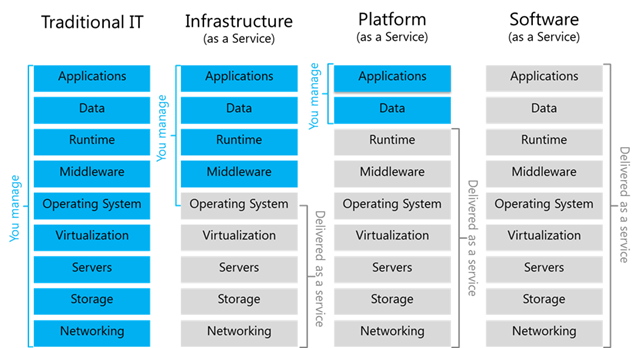
\includegraphics[width=1.0\textwidth]{fig/aa-hauptteil/Service-Models.png}

	\caption{Die Cloud Service Modelle im �berblick\cite{svc-mod}}

	\centering

\end{figure}

\textbf{Infrastructure as a Service:} Der Nutzer hat die F�higkeit Rechenleistung, Datenspeicher
 Netzwerke und weitere fundamentale Computing Ressourcen bereitzustellen und beliebige Software
 darauf zu betreiben, dazu k�nnen Betriebssysteme und Anwendungen geh�ren. Die
darunterliegende Infrastruktur wird vom Anbieter betrieben, der Nutzer kann aber
eingeschr�nkte Kontrolle �ber bestimmte Komponenten haben, dazu geh�ren beispielsweise
Firewalls.


\textbf{Platform as a Service:} Der Nutzer verf�gt �ber die F�higkeit seine eingekaufte oder
selbst erstellten Anwendungen auf der Cloud Infrastruktur zu betreiben, die notwendige
Umgebung die �ber Sprachen, Bibliotheken, Tools und Services verf�gt wird vom Cloud Service Provider (CSP) bereitgestellt. Die darunter liegende Infrastruktur mit Netzwerken, Servern,
Betriebssystemen und Speicher wird vom CSP betrieben, der Nutzer hat die Kontrolle
�ber Anwendung und Konfiguration der Umgebung in der die Anwendung betrieben wird.


\textbf{Software as a Service:} Dem Nutzer wird der Zugriff auf die vom CSP in der
Cloud Infrastruktur betriebenen Softwareanwendung gew�hrt. Auf diese wird mithilfe
eines Thin oder Fat Client zugegriffen, dabei k�mmert sich der Nutzer nicht um den
Betrieb und die Konfiguration der darunterliegenden Cloud Infrastruktur (Netzwerke, Server, Betriebssystem, Speicher) und die Anwendung selbst mit Ausnahme
eingeschr�nkter Nutzereinstellungen.\\

In Art der Bereitstellung eines Cloud Services werden vier grundlegende Modelle
unterschieden; es existieren Public, Private, Hybrid und Community Cloud Modelle.\\


\textbf{Private Cloud}: Die Cloud Infrastruktur wird ausschlie�lich f�r die Nutzung durch eine einzige
Organisation mit mehreren Nutzern bereitgestellt. Besitz und Betrieb liegen dabei
entweder bei der selben Organisation, einer Drittpartei oder einer Kombination beider, die Infrastruktur kann dabei On- oder Off-Premises\footnote{Hardware ist lokal vor Ort/nicht vor Ort} betrieben werden.

\textbf{Public Cloud}: Die Public Cloud steht f�r die Nutzung durch die allgemeine �ffentlichkeit bereit.
Die Cloud Infrastruktur befindet sich im Besitz eines Unternehmens, Bildungseinrichtung,
Regierungsorganisation oder einer Kombination aus diesen und wird auch von der selben
 Organisation On-Premises betrieben. 


\textbf{Community Cloud}: Eine Community Cloud wird von einer Gemeinschaft von Nutzern mit gemeinsamen
Anliegen eingesetzt. Der Besitz und Betrieb liegen dabei bei einem oder mehreren
Mitgliedern dieser Gemeinschaft, einer Drittpartei und kann Off- oder On-Premises betrieben

werden.


\textbf{Hybrid Cloud}: Die Hybrid Cloud besteht aus einer Kombination der beschriebenen Modelle (Public, Private und Community). Diese bilden dabei eigene Instanzen die aber durch standardisierte oder propriet�re Schnittstellen den Transfer von Daten und Anwendungen
zwischen den Instanzen erlauben.

\subsection{Vor- und Nachteile des Einsatzes von Cloud Computing}

\subsubsection{Vorteile und Treiber der Adoption von Cloud Computing}

\textbf{Wirtschaftliche Vorteile}: Ein Vorteil in der Nutzung von Cloud Computing
kann darin liegen dass ein Gro�teil der f�r den Betrieb notwendigen Infrastruktur
nicht mehr vom Unternehmen selbst eingekauft, eingerichtet und betrieben werden
muss (Abb. 2.1). Potentiell hohe Kosten die bereits vor der
Inbetriebnahme eines Systems mit einem h�heren Risiko aufgewendet werden m�ssen
stellen in Form von individuell geringeren laufenden Betr�gen ein deutlich
reduziertes Risiko dar\cite{capex-opex}.\\
Sofern der Einsatz von Cloud Computing in einer sinnvollen und korrekten
Weise erfolgt k�nnen je nach Fall die Gesamtkosten um einen hohen Anteil reduziert
werden\cite{total-cost}.\\
Die Gesamtkostenersparnisse stehen auch im Zusammenhang mit Skaleneffekten\footnote{Zusammenhang zwischen produziertem Ertrag und eingesetzter Ressourcen} die f�r
gro�e Cloud Service Provider gelten. Der Betrieb eines einzelnen Servers ist im Verh�ltnis
mit bedeutend h�heren Kosten verbunden als das hinzuf�gen eines �quivalenten
Systems zu einem Rechenzentrum im Betrieb von Mircosoft oder einem vergleichbaren
Anbieter\cite{econ-scale}.

\textbf{Skalierbarkeit}: Besonders f�r schnell wachsende Unternehmen ist die
M�glichkeit schneller Skalierbarkeit einer der prominentesten Vorteile der Cloud.
Es kann nicht nur auf vorhersagbare Anstiege (zum Beispiel ausgel�st durch
eine Verkaufsaktion) sondern auch auf unvorhersehbare Ereignisse reagiert werden.
Zus�tzlich ist es m�glich diese Skalierung nicht nur bis zu einem bestimmten Limit,
sondern nahezu unendlich zu betreiben. Wichtig ist auch dass sowohl auf steigende
als auch sinkende Nachfrage reagiert werden kann\cite{scale}.

\textbf{Resilienz}: In einem Worst Case-Szenario kann ein ganzes Rechenzentrum
durch unvorhergesehen Ereignisse wie beispielsweise Br�nde, Naturkatastrophen
oder anderes vollst�ndig zerst�rt werden. Selbst wenn Backup-Rechenzentren
verf�gbar sind ist eine �bertragung der Operationen kein trivialer Ablauf und
birgt oft nicht au�er Acht zu lassende Risiken. Die Flexibilit�t der Cloud
erlaubt es die gesamte Infrastruktur mit sehr geringem Aufwand in nicht
betroffene Regionen zu verlagern und die Kontinuit�t der Gesch�ftst�tigkeiten
mit minimaler Unterbrechung aufrecht zu erhalten\cite{resil}.

\textbf{Security}: Sicherheitsaspekte k�nnen sowohl einen Vor- als auch Nachteil
von Cloud Computing darstellen. Hier sollen zuerst Vorteile dargelegt werden,
potentielle Probleme sind im n�chsten Abschnitt beschrieben.\\
Die technischen M�glichkeiten und besonders auch die Wahrnehmung des Themas
Sicherheit in der Cloud unterlagen und unterliegen auch noch immer einem
deutlichen Wandel. Cloud Anbieter investieren
viele Ressourcen in Sicherheit und stellen dem Nutzer zum Beispiel bereits sicher
implementierte Verschl�sselungen zur Verf�gung oder bieten einen gewissen
Schutz vor Denial-of-Service Angriffen durch ihre \enquote{nat�rliche} Skalierbarkeit\cite{sec-1}.

\subsubsection{Herausforderungen und Risiken}

\textbf{Netzwerkabh�ngigkeit}: Da der Zugriff auf Cloud Dienste �ber das
Internet erfolgt entsteht dadurch entsprechend auch eine hohe Abh�ngigkeit. Stabile und schnelle Netzwerkanbindung ist eine kritische Voraussetzung f�r effektives Arbeiten\cite{net-dep}, bei lokal gehosteten Systemen ist diese Abh�ngigkeit
entsprechend geringer.

\textbf{Vendor Lock-in}: Bei der Nutzung eines Cloud Anbieters entsteht die
Gefahr sich zu sehr in Abh�ngigkeit eines einzelnen Anbieters zu begeben.
Im Fall einer �nderung der Nutzungsbedingungen oder einer �nderung im
Kostenmodell die den eignen Interessen stark entgegen steht, besteht die Gefahr
bereits so abh�ngig von diesem Anbieter zu sein dass die Kosten eines Wechsels
derart hoch ausfallen dass man gezwungen ist die Bedingungen zu akzeptieren\cite{lock-in}.

\textbf{Security und Privacy}: Sicherheitsrisiken sind einer der meistgenannten
Gr�nde die gegen Cloud Computing sprechen\cite{sec-2}, besonders im Fall der Nutzung einer
Public Cloud. Die Gefahr dass Daten in die H�nde dritter gelangen kann zum
beispielsweise nicht vollst�ndig ausgeschlossen werden. Da die Verantwortung �ber
die Sicherheit der Daten dem Cloud Anbieter unterliegt kann es auch zu Problemen
hinsichtlich Privatheit der Daten kommen, sollte etwa eine Regierungsorganisation
Zugriff auf bestimmte Daten eines Nutzer verlangen k�nnte dieser ohne dessen
Einverst�ndnis gew�hrt werden.

\textbf{Kosten}: Auch wenn die Nutzung von Cloud Computing mit dem Vorteil
geringerer Kosten beworben wird, ist dies nicht zwingend garantiert. Werden die
vorhandenen Systeme ung�nstig verwendet, bleiben zum Beispiel viele gebuchte
CPUs und IP-Adressen sowie weitere Ressourcen ungenutzt, k�nnen unn�tig hohe Kosten entstehen. Auch w�hrend der Migrationsphase, in der m�glicherweise beide Systeme parallel betrieben werden m�ssen, k�nnen h�here Kosten
entstehen als in einem vergleichbaren Zeitraum davor. Nicht zuletzt stellt die Migration komplexer Systeme h�ufig eine gro�e technische und dadurch auch finanzielle Herausforderung dar\cite{migration-cost}.

\subsection{�berblick �ber die wichtigsten Public Cloud Service Provider}

In diesem Abschnitt soll ein knapper �berblick �ber die wichtigsten Public Cloud Service Provider gegeben werden.

\section{Stand der Technik}

\subsection{Eingesetzte Technik zur Realisierung eines Konzepts als Cloud-basierte Software}

\section{Infrastructure as Code}

\subsection{Technologischer Wandel und das Cloud Age Mindset}

\subsection{Vorteile von Infrastructure as Code im Vergleich zu manuellem Infrastruktur-Provisioning}

\subsection{Herausforderungen im Einsatz von Infrastructure as Code}

\subsection{Die drei Kernverfahren von Infrastructure as Code}

\section{Funktionsprinzip und Rolle von Terraform im IaC-Anwendungsprozess}

\subsection{Funktionsweise von Terraform}

\subsection{�berblick �ber die Hashicorp Configuration Language}




\chapter{Evaluierungsanforderungen und Umsetzung}
\label{sec:ergeb}

\section{Evaluierungsanforderungen}

\subsection{Ziel der Evaluierung}

\subsection{Untersuchte Komponenten der Terraform Provider}

\subsection{Auswahl der Evaluierungskriterien}




\section{Umsetzung des Testsystems}

\subsection{Eingesetzte Software und Tools}

\subsection{High-Level Aufbau des Testsystems}

\subsection{Konkreter Aufbau auf Google Cloud Platform}

\subsection{Konkreter Aufbau auf Azure}

\subsection{Aufbau der erg�nzenden Versuche}




\chapter{Ergebnisse und Bewertung}

\section{Evaluierung der Functional Completeness}

\section{Ergebnisse und Bewertung der Time Behaviour Tests}

\section{Ergebnisse und Bewertung der Recoverability Tests}

\section{Ergebnisse und Bewertung der Modifiability Tests}

\section{Evaluierung der Einheitlichkeit der Testsysteme f�r Azure und Google Cloud Platform}





\begin{spacing}{1.2}

\chapter{Schluss}
\label{sec:schluss}

\section{Zusammenfassung der Arbeit}

Im Rahmen dieser Arbeit wurde ein Vergleich der Public Cloud Service
Provider Google Cloud Platform und Microsoft Azure in Bezug auf die
Unterstützung von Infrastructure as Code mit Terraform durchgeführt.
Um den Kontext, die technischen Grundlagen und die Motivation der Arbeit
darzustellen werden im ersten Abschnitt Funktionsprinzip, Vorteile und
Herausforderungen des modernen Cloud Computings sowie die Grundlagen
von Infrastructure as Code und Terraform zusammengefasst.
Grundlage für die Erklärung des Funktionsprinzip von Cloud Computing
stellt hierbei die weithin akzeptierte Definition des National
Institude of Standards and Technology der USA dar.
Dazu werden verschiedene Vorteile und Herausforderungen moderner Cloud
Technologien kurz zusammengefasst und erläutert sowie ein
Überblick über die wichtigsten Cloud Service Provider im aktuellen
Markt hergestellt.

Die Grundlagen zu Infrastructure as Code werden durch den
technologischen Wandel und eine Erklärung des Cloud Age Mindset
eingeleitet. Die Notwendigkeit für den Einsatz von IaC wird durch
die bestehenden Probleme welche durch IaC gelöst werden dargestellt,
und drei Kernverfahren im Einsatz von IaC erläutert.
Zum Abschluss der Grundlagen wird das IaC Tool Terraform vorgestellt.
Es wird das Einsatzfeld von Terraform im Rahmen von IaC dargestellt
sowie die Funktionsweise von Terraform und die von Terraform
verwendete Sprache erläutert.

Der Hauptteil der Arbeit beschäftigt sich mit der Auswahl der 
Evaluierungskriterien, dem Aufbau des primären Testsystems und
der Definition und Durchführung von zusätzlichen ergänzenden Tests.\\
Die Evaluierungskriterien werden aus dem Qualitätsmodell der ISO
25010 ausgewählt, die individuellen Qualitätsaspekte werden hinsichtlich
ihrere Anwendbarkeit beurteilt und geeignete Aspekte zur Untersuchung
ausgewählt.

Der nächste Teil besteht aus der Vorstellung des primären Testsystems.
Dieses besteht aus drei Terraform-Modulen; dem Root-Modul sowie
zwei nach ihrer Funktionlität getrennten Modulen für einen 
Datenbankserver und einem Kubernetes Cluster.

Dieses System sowie die zusätzlichen Tests werden hinsichtlich der zuvor
ausgewählten Qualitätsmerkmale verglichen und bewertet.

Der letzte Abschnitt der Arbeit umfasst eine Zusammenfassung, 
das abschließende Fazit sowie einen Ausblick auf weitere
untersuchenswerte Themen im Zusammen mit Infrastructure as Code
und Terraform. 

\section{Fazit}

Abschließend lässt sich die Aussage treffen dass sowohl Google Cloud
Plattform als auch Microsoft Azure gut für den Einsatz von Infrastructure
as Code mit Terraform geeignet sind. Beide Terraform Provider befinden
sich in einem ausgereiften Zustand, grundlegend fehlende
Funktionalitäten wurden im Rahmen dieser Evaluierung nicht festgestellt.
Betrachtet man die Details macht Microsoft Azure insgesamt eine
leicht bessere Figur. Die Deployment Zeiten sind im Durchschnitt
etwas schneller und es existieren einige Funktionalitäten die von
Google Cloud Platform aktuell noch nicht vollständig abgedeckt sind.
Die Dokumentation der Terraform Provider beider Cloud Plattformen
fällt sehr gut und umfangreich aus, inklusive einiger Beispiele wie
die individuellen Ressourcen konfiguriert werden können bzw. müssen.

\section{Weitere untersuchenswerte Aspekte und aktuelle Entwicklungen}

Im Verlauf dieser Arbeit wurden eine Vielzahl von Themen angeschnitten
oder erwähnt die für die Umsetzung eines kundenorientierten Projekts
mitunter große Relevanz besitzen, aufgrund des inhaltlichen und
zeitlichen Rahmens jedoch nicht adäquat behandelt werden konnten.\\
Das vielleicht wichtigste dieser Themen ist das Testen von Infrastruktur
Code. Interessant wäre hier nicht nur die Untersuchung der existierenden
Möglichkeiten von Terraform sondern auch der Vergleich mit anderen
Tools wie Pulumi. Allgemein wäre nicht nur der Vergleich der
Testmöglichkeiten interessant, eine grundsätzliche Evaluierung beider
Tools könnte interessante Erkentnisse über die Eignung dieser
in verschiedenen Szenarien liefern und verschiedene Aspekte beider Tools
genauer betrachten.\\
Ein weiteres interessantes Thema ist die Cloud Agnostizität von
Terraform. Das Erfassen des Unterschieds zwischen Erwartung und Realität
sowie das Erforschen der bestehenden Möglichkeiten zum Erreichen einer
\enquote{echten} Cloud Agnostizität in Form einer fundierten Arbeit
wäre mit Sicherheit eine wertvolle Referenz für Neueinsteiger in das
Thema IaC mit Terraform.\\
Im Grundlagenkapitel dieser Arbeit wurde dargestellt warum die
Automatisierung von Infrastruktur von Beginn an essentiell ist um
den vollen Umfang der Vorteile ausschöpfen zu können. Ein Großteil
der aktuell existierenden Projekte ist jedoch aufgrund der
verhältnismäßigen Neuheit von IaC und Terraform mit hoher
Wahrscheinlichkeit noch nicht in dieser Form umgesetzt worden.
Eine Erforschung von Best Practices und Tools zur Automatisierung
bestehender Systeme hätte zum aktuellen Zeitpunkt und auch in
kommenden Jahren einen hohen Wert.\\

\end{spacing}


% % %%%%%% Anhang
\appendix
\chapter{Kapitel im Anhang}
\label{sec:a-kapitel}

Alles was den Hauptteil unnötig vergrößert hätte, z. B. HW-/SW-Dokumentationen, Bedienungsanleitungen, Code-Listings, Diagramme


% % %%%%%% Literaturverzeichnis (darf im deutschen nicht in den Anhang!)
% Einfaches Literaturverzeichnis
\begin{thebibliography}{XXXX}

\bibitem{verbr-cloud} Asadi, S., Nilashi, M., Husin, A.R.C. et al. -  Customers perspectives on adoption of cloud computing in banking sector. Inf Technol Manag 18, 305?330 (2017). [Online] Verf�gbar unter: \url{https://doi.org/10.1007/s10799-016-0270-8} (Zugriff am: 23.01.2022)

\bibitem{def-cloud} Mell, Peter, and Tim Grance. - "The NIST definition of cloud computing." (2011). [Online] Verf�gbar unter: \url{http://faculty.winthrop.edu/domanm/csci411/Handouts/NIST.pdf} (Zugriff am: 28.10.2021)

\bibitem{svc-mod} Chou, David. Cloud Service Models (IaaS, PaaS, SaaS) Diagram (2018). [Online] Verf�gbar unter: \url{https://dachou.github.io/2018/09/28/cloud-service-models.html} (Zugriff am: 28.10.2021)

\bibitem{capex-opex} Lisdorf, Anders. - Cloud computing basics a non-technical introduction. Berkeley, CA: Apress, 2021. S.23.

\bibitem{total-cost} Lisdorf, Anders. - Cloud computing basics a non-technical introduction. Berkeley, CA: Apress, 2021. S.24.

\bibitem{econ-scale} Lisdorf, Anders. - Cloud computing basics a non-technical introduction. Berkeley, CA: Apress, 2021. S.24-25.

\bibitem{scale} Lisdorf, Anders. - Cloud computing basics a non-technical introduction. Berkeley, CA: Apress, 2021. S.27.

\bibitem{resil} Lisdorf, Anders. - Cloud computing basics a non-technical introduction. Berkeley, CA: Apress, 2021. S.26.

\bibitem{sec-1} Lisdorf, Anders. - Cloud computing basics a non-technical introduction. Berkeley, CA: Apress, 2021. S.25.

\bibitem{net-dep} NANDGAONKAR, Suruchee V.; RAUT, A. B. A comprehensive study on cloud computing. International Journal of Computer Science and Mobile Computing, 2014, 3. Jg., Nr. 4, S. 737.

\bibitem{sec-2} NANDGAONKAR, Suruchee V.; RAUT, A. B. A comprehensive study on cloud computing. International Journal of Computer Science and Mobile Computing, 2014, 3. Jg., Nr. 4, S. 737.

\bibitem{lock-in} OPARA-MARTINS, Justice; SAHANDI, Reza; TIAN, Feng. Critical analysis of vendor lock-in and its impact on cloud computing migration: a business perspective. Journal of Cloud Computing, 2016, 5. Jg., Nr. 1, S. 1-18. [Online] Verf�gbar unter \url{https://ieeexplore.ieee.org/abstract/document/7009018} (Zugriff am: 24.01.2022)

\bibitem{migration-cost} BAI, Kun, et al. What to discover before migrating to the cloud. In: 2013 IFIP/IEEE International Symposium on Integrated Network Management (IM 2013). IEEE, 2013. S. 320. [Online] Verf�gbar unter: \url{https://ieeexplore.ieee.org/stamp/stamp.jsp?tp=&arnumber=6573001} (Zugriff am: 24.01.2022)

\bibitem{csp-share} Kein Autor. Enterprise spending on cloud infrastructure services grows to USD 42 billion in Q2, 2021: SRG (2021) [Online] Verf�gbar unter: \url{https://www.cioandleader.com/article/2021/07/30/enterprise-spending-cloud-infrastructure-services-grows-usd-42-billion-q2-2021} (Zugriff am: 24.01.2022)

\bibitem{gartner-mag} Bala, Raj; Gill, Bob; Smith, Dennis; Ji, Kevin; Wright, David. Magic Quadrant for Cloud Infrastructure and Platform Services (2021) [Online] Verf�gbar unter: \url{https://www.gartner.com/doc/reprints?id=1-271OE4VR&ct=210802&st=sb} (Zugriff am: 24.01.2022)

\bibitem{def-iac} Kief Morris. Infrastructure as Code. O?Reilly Media, 2. edition, 2020. S.4

\bibitem{dec-imp-iac} Jacobs, Mike; Kaim, Ed. What is Infrastructure as Code? (2021) [Online] Verf�gbar unter: \url{https://docs.microsoft.com/en-us/devops/deliver/what-is-infrastructure-as-code} (Zugriff am: 24.01.2022)

\bibitem{iac-schneller} Kief Morris. Infrastructure as Code. O?Reilly Media, 2. edition, 2020. S.3

\bibitem{conf-drift} Kief Morris. Infrastructure as Code. O?Reilly Media, 2. edition, 2020. S.17-18

\bibitem{cattle-pets} Kief Morris. Infrastructure as Code. O?Reilly Media, 2. edition, 2020. S.16

\bibitem{opt-change} Kief Morris. Infrastructure as Code. O?Reilly Media, 2. edition, 2020. S.4-5

\bibitem{stab-cloud} Kief Morris. Infrastructure as Code. O?Reilly Media, 2. edition, 2020. S.5

\bibitem{build-auto} Kief Morris. Infrastructure as Code. O?Reilly Media, 2. edition, 2020. S.6

\bibitem{speed-quality} Kief Morris. Infrastructure as Code. O?Reilly Media, 2. edition, 2020. S.8

\bibitem{coreprinc-1} Kief Morris. Infrastructure as Code. O?Reilly Media, 2. edition, 2020. S.10

\bibitem{coreprinc-2} Kief Morris. Infrastructure as Code. O?Reilly Media, 2. edition, 2020. S.11

\bibitem{iac-tools} Nayak, Ramnath. When to use which Infrastructure-as-code tool (2019) [Online] Verf�gbar unter: \url{https://medium.com/cloudnativeinfra/when-to-use-which-infrastructure-as-code-tool-665af289fbde} (Zugriff am: 25.01.2022)

\bibitem{tf-princ} Terraform Website. [Online] Verf�gbar unter: \url{https://www.terraform.io/} (Zugriff am: 25.01.2022)

\bibitem{hcl} Introduction to HashiCorp Configuration Language (HCL). [Online] Verf�gbar unter: \url{https://www.linode.com/docs/guides/introduction-to-hcl/} (Zugriff am: 25.01.2022)

\bibitem{tf-provider} Terraform Provider Documentation. [Online] Verf�gbar unter: \url{https://www.terraform.io/language/providers} (Zugriff am: 26.01.2022)

\bibitem{tf-state} Terraform State Documentation. [Online] Verf�gbar unter: \url{https://www.terraform.io/language/state/purpose} (Zugriff am 26.01.2022)

\bibitem{tf-workflow} Kumar, Rajesh. Terraform Basics Workflow loop explained!!! (2019). [Online] Verf�gbar unter: \url{https://www.devopsschool.com/blog/terraform-basics-workflow-loop-explained/} (Zugriff am: 26.01.2022)

\end{thebibliography}
% Literaturverzeichnis mit Bibtex
%\bibliography{bib/bib}

% %  Inhalt ENDE %%%%%%%%%%%%%%%%%%%%%%%%%%%%%%%%%%%%%%%%%%%%%%%%%%%%%%%%%%
\end{document}
